\documentclass{article}
\usepackage{amsmath}
\usepackage{graphicx}
\usepackage{subfig}


\begin{document}
\title{PP2 Report}
\author{Logan Bontrager}
\maketitle

\section*{Task 1)}

In task one, we are comparing bayesian linear regression to linear regression with and without regularization. To do this, we train models on various fractions of data and evaluate the mean squared error on unseen data. Note the models are built using the closed form solution for maximum likelihood and the model selection algorithm. 
\\ \\
The following graphs depicts each model's performance on the artificial and crime datasets.

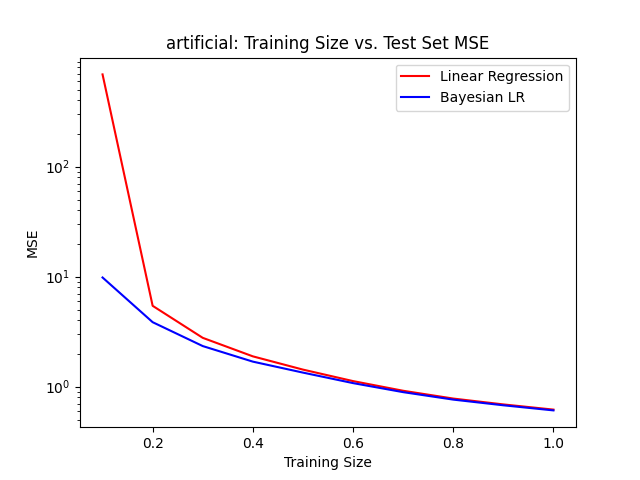
\includegraphics[width=0.5\textwidth]{../output/task1iiartificial.png}
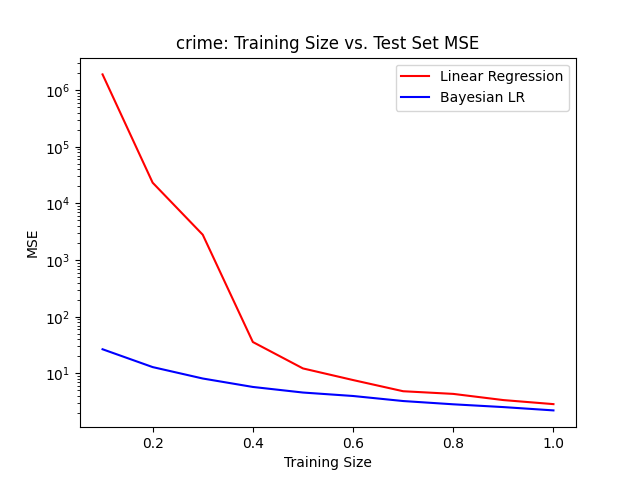
\includegraphics[width=0.5\textwidth]{../output/task1iicrime.png}
Here, we can see that the bayesian linear regression with the model selection algorithm performs much better on small fractions of training data then normal linear regression. This is expected with a well choosen prior as the model will better approximate the true underlying distribution. Another thing to note is that the mse for linear regression decends faster on the aritficial dataset than the crime dataset in relation to training size. Thus, results are both very model and data specific.
\\ \\
Next, we repeat this process using set values for lambda, specifically 1, 33, and 1000, in our bayesian linear regression.

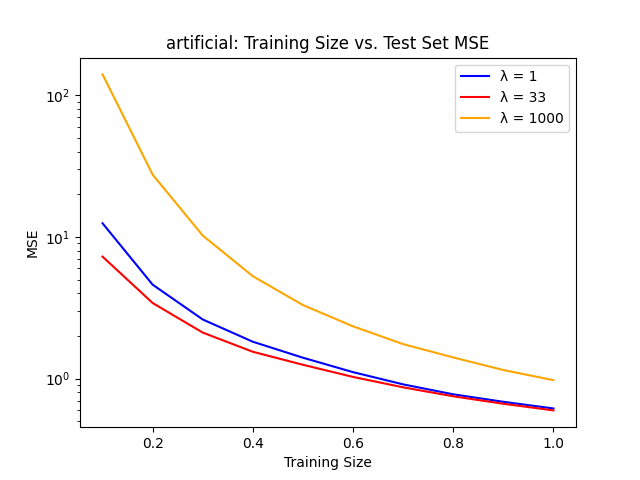
\includegraphics[width=0.5\textwidth]{../output/task1iiiartificial.png}
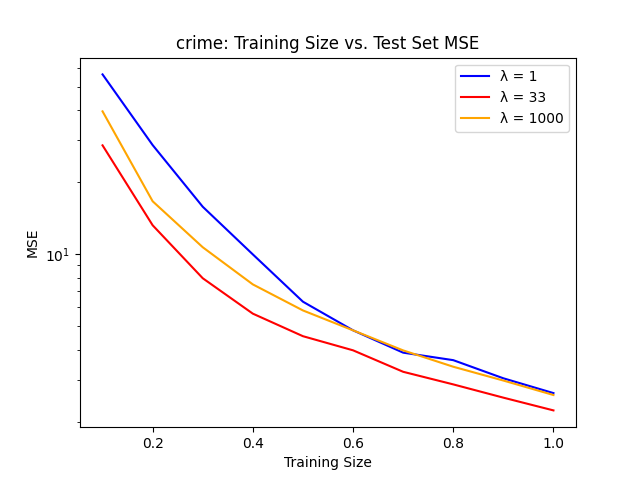
\includegraphics[width=0.5\textwidth]{../output/task1iiicrime.png}
From the graphs and code output, it is apparent that there isn't a specific lambda value that minimizes the mean squared error. Notice that the relative performance for the specific lambda values is not consistent across both sets of data. It appears that the best lambda much be chosen in relevance to given data. In terms of the bayesian model, the model selection algorithm chooses lambda values of approximately 5 for the artifical dataset and 120 for the crime dataset. This was taken from the code output which is located at the end of this report. For good measure, I also created graphs including these lambda values which are given below.

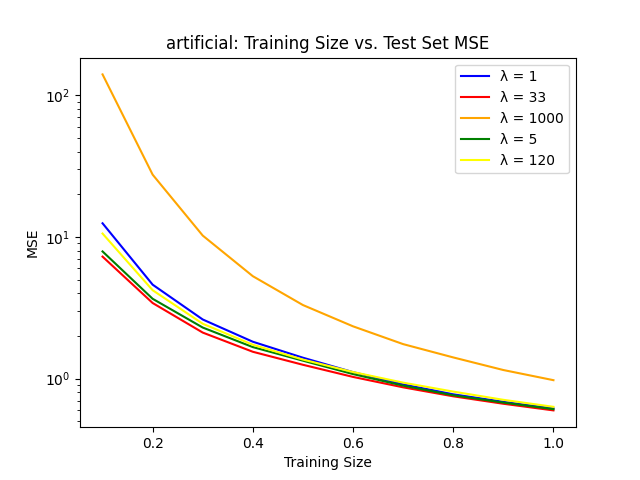
\includegraphics[width=0.5\textwidth]{../output/task1iiiartificialcopy.png}
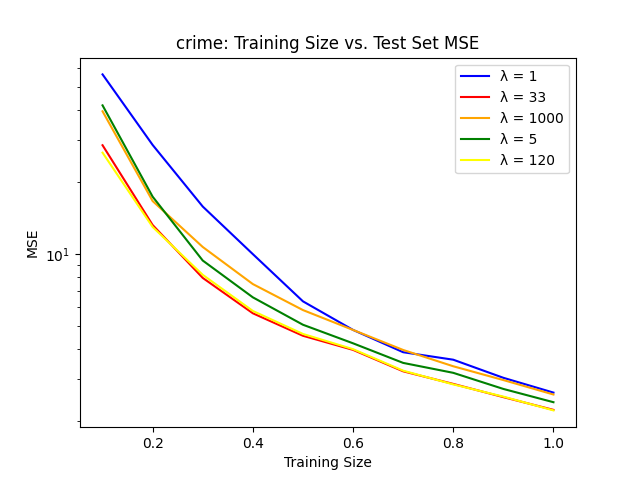
\includegraphics[width=0.5\textwidth]{../output/task1iiicrimecopy.png}
It is interesting to see that both values selected using the model selection algortihm perform well relative to the others, but not necessarily the best. Thus, we could potentially conclude that the algorithm does not always select the best lambda and there may be another way to choose a lambda value that gives better results. Although given the unknown training and test dataset discrepancy it is hard to know in this given context. Note that another way to select the regularization parameter could be gradient descent.

\section*{Task 2)}

In task two, we test the bayesian and linear models on data generated with polynomials. The following graphs show the degree of the model versus the mean squared error of the trained model tested on external data.

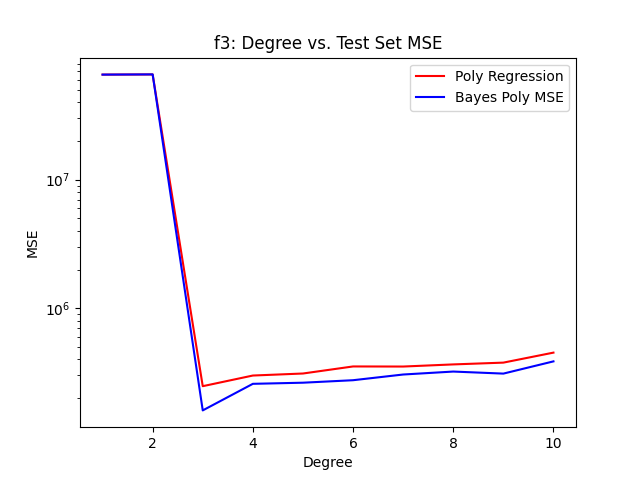
\includegraphics[width=0.5\textwidth]{../output/task2f3.png}
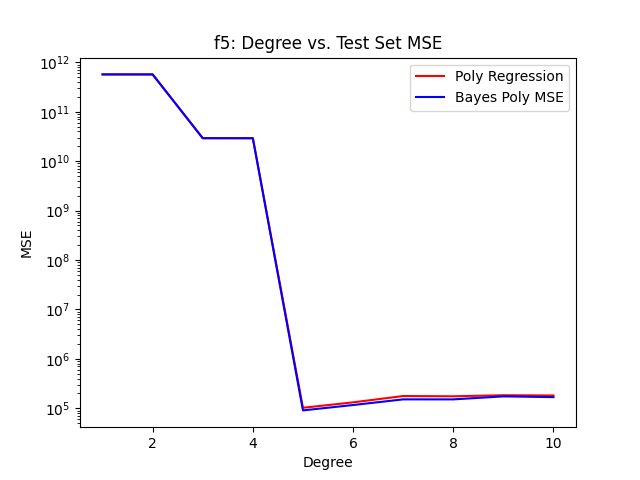
\includegraphics[width=0.5\textwidth]{../output/task2f5.png}
We see that the error is minimized for the model which uses the same degree as the polynomial used to generate the data which is 3 and 5 respectively. Next, we plot the degree of the model against the log evidence.

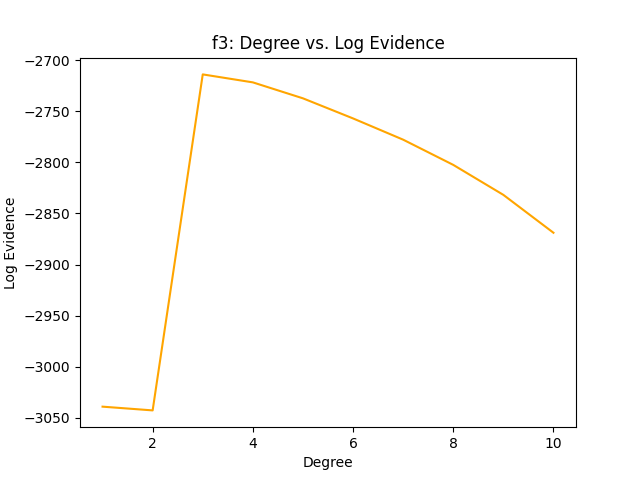
\includegraphics[width=0.5\textwidth]{../output/task2f3evid.png}
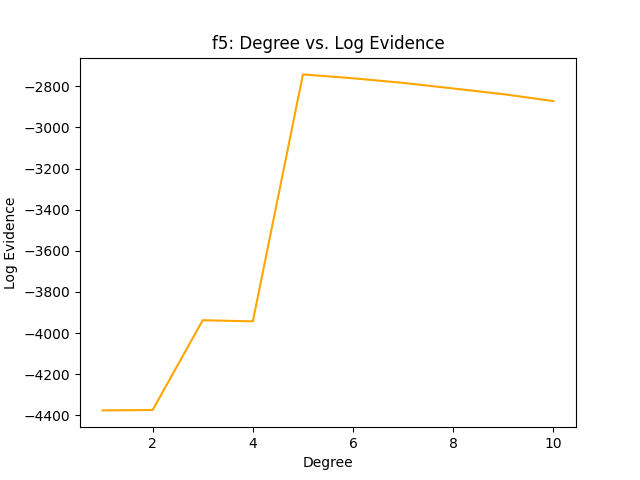
\includegraphics[width=0.5\textwidth]{../output/task2f5evid.png}
As expected the log evidence is maximized for the same respective degrees as the polynomials used to generate the data. Thus, the evidence could be used to select values for alpha, beta, and the degree of the model. Note that the non-regularized regression performs relatively well on this. 

\end{document}